% Options for packages loaded elsewhere
\PassOptionsToPackage{unicode}{hyperref}
\PassOptionsToPackage{hyphens}{url}
%
\documentclass[
]{article}
\usepackage{amsmath,amssymb}
\usepackage{iftex}
\ifPDFTeX
  \usepackage[T1]{fontenc}
  \usepackage[utf8]{inputenc}
  \usepackage{textcomp} % provide euro and other symbols
\else % if luatex or xetex
  \usepackage{unicode-math} % this also loads fontspec
  \defaultfontfeatures{Scale=MatchLowercase}
  \defaultfontfeatures[\rmfamily]{Ligatures=TeX,Scale=1}
\fi
\usepackage{lmodern}
\ifPDFTeX\else
  % xetex/luatex font selection
\fi
% Use upquote if available, for straight quotes in verbatim environments
\IfFileExists{upquote.sty}{\usepackage{upquote}}{}
\IfFileExists{microtype.sty}{% use microtype if available
  \usepackage[]{microtype}
  \UseMicrotypeSet[protrusion]{basicmath} % disable protrusion for tt fonts
}{}
\makeatletter
\@ifundefined{KOMAClassName}{% if non-KOMA class
  \IfFileExists{parskip.sty}{%
    \usepackage{parskip}
  }{% else
    \setlength{\parindent}{0pt}
    \setlength{\parskip}{6pt plus 2pt minus 1pt}}
}{% if KOMA class
  \KOMAoptions{parskip=half}}
\makeatother
\usepackage{xcolor}
\usepackage[margin=1in]{geometry}
\usepackage{graphicx}
\makeatletter
\def\maxwidth{\ifdim\Gin@nat@width>\linewidth\linewidth\else\Gin@nat@width\fi}
\def\maxheight{\ifdim\Gin@nat@height>\textheight\textheight\else\Gin@nat@height\fi}
\makeatother
% Scale images if necessary, so that they will not overflow the page
% margins by default, and it is still possible to overwrite the defaults
% using explicit options in \includegraphics[width, height, ...]{}
\setkeys{Gin}{width=\maxwidth,height=\maxheight,keepaspectratio}
% Set default figure placement to htbp
\makeatletter
\def\fps@figure{htbp}
\makeatother
\setlength{\emergencystretch}{3em} % prevent overfull lines
\providecommand{\tightlist}{%
  \setlength{\itemsep}{0pt}\setlength{\parskip}{0pt}}
\setcounter{secnumdepth}{-\maxdimen} % remove section numbering
\usepackage{float}
\usepackage{caption}
\captionsetup{labelformat=empty}
\ifLuaTeX
  \usepackage{selnolig}  % disable illegal ligatures
\fi
\IfFileExists{bookmark.sty}{\usepackage{bookmark}}{\usepackage{hyperref}}
\IfFileExists{xurl.sty}{\usepackage{xurl}}{} % add URL line breaks if available
\urlstyle{same}
\hypersetup{
  pdftitle={Appendix: Minimum and maximum for range of counterfactual household counts},
  hidelinks,
  pdfcreator={LaTeX via pandoc}}

\title{Appendix: Minimum and maximum for range of counterfactual
household counts}
\author{}
\date{\vspace{-2.5em}}

\begin{document}
\maketitle

\hypertarget{definitions-and-notation}{%
\section{Definitions and Notation}\label{definitions-and-notation}}

Let:

\begin{itemize}
\item
  \(P\) = \textbf{Total population size}
\item
  \(H\) = \textbf{Number of households}
\item
  \(M_p\) = \textbf{Person-level mean household size}

  For every person \(j\) in a population \(P\) living in a household of
  \(m_j\) members, the \textbf{person-level} mean household size is a
  simple average across person-level observations:

  \begin{equation}
    \label{eq:1}
    \tag{1}
    M_p = \frac{1}{P} \sum_{j = 1}^H m_j^2
    \end{equation}
\item
  \(M_h\) = \textbf{Household-level mean household size}

  The \textbf{household-level} mean household size is a simple average
  across households as individual observations:

  \begin{align}
    \label{eq:2}
    \tag{2}
    M_h = \frac{P}{H}
    \end{align}
\end{itemize}

\begin{center}\rule{0.5\linewidth}{0.5pt}\end{center}

\hypertarget{context}{%
\section{Context}\label{context}}

Equation \eqref{eq:2} shows that household-level mean household size
\(M_h\) and population \(P\) is adequate to deduce the number of
households \(H\). However, person-level household size \(M_p\) does not
lend itself to this equivalency: the same person-level mean and
population can be consistent with multiple values for the number of
households.

Figure 1.2 illustrates this point in a hypothetical population with
\(P = 6\) and \(M_p = 3\). In Scenario 1, average person-level household
size is \(\frac{3^2 + 3^2}{6} = 3\) and there are 2 households. In
Scenario 2, average person-level household size is
\(\frac{1^2 + 1^2 + 4^2}{6} = 3\) and there are 3 households. Thus,
population and person-level household size alone do not singularly
determine the number of households.

\textbf{Figure 1.2}

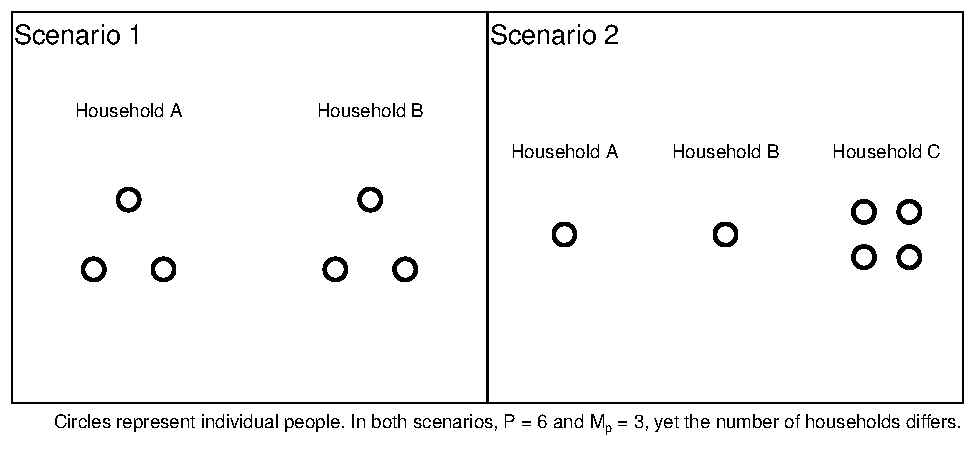
\includegraphics[width=1\linewidth]{proof_files/figure-latex/unnamed-chunk-1-1}

\begin{center}\rule{0.5\linewidth}{0.5pt}\end{center}

\hypertarget{assertion}{%
\section{Assertion}\label{assertion}}

There is a range of possible number of households \(H\) consistent with
a known population size \(P\) and person-level average household size
\(M_p\). The range on \(H\) is bounded by a minumum of

\begin{align}
H_{min} = \frac{P}{M_p}
\end{align}

and a maximum of

{[}FILL IN HERE{]}

\begin{center}\rule{0.5\linewidth}{0.5pt}\end{center}

\hypertarget{lemma-1-minimum-number-of-households}{%
\section{Lemma 1: Minimum Number of
Households}\label{lemma-1-minimum-number-of-households}}

The minimum number of households consistent with a population size \(P\)
and person-level average household size \(M_p\) is: \begin{align}
H_{\min} = \frac{P}{M_p}
\end{align}

\hypertarget{proof}{%
\subsection{Proof}\label{proof}}

Suppose the population \(P\) is distributed into \(H\) households with
the measured household size in the \(j\)th household equal to \(m_j\).
As defined above, \textbf{person-level} mean household size is:

\begin{equation}
M_p = \frac{1}{P}\sum_{j = 1}^H m_j^2
\end{equation}

Any configuration of \(P\) individuals across households can be
transformed into any other configuration through a finite sequence of
single-person transfers. The initial count of households, \(H\), need
not match the final count of households, \(H'\): we conceptualize a
`reservoir' of zero-person households to account for changes between
\(H\) and \(H'\). Forming a new household can be conceptualized as
moving an individual to a zero-person household, which remains uncounted
unless populated. Conversely, a household can be dissolved by moving all
of its members to other households, thus turning a household with a
positive number of members into a zero-person household. For example, in
Figure 1.2, once can incrementally create Scenario 2 after starting from
Scenario 1 through the following steps:

\begin{enumerate}
\def\labelenumi{\arabic{enumi}.}
\tightlist
\item
  Move one individual from Household A to a newly formed Household C.
\item
  Move another individual from Household A to Household C.
\item
  Move two individuals from Household B to Household C.
\end{enumerate}

Next, we calculate how the person-level mean household size changes
after a single-person transfer. Suppose we begin with an arbitrary
configuration of \(P\) individuals in \(H\) households, with each
household \(m_j\) containing some whole number of members
\(m_1, m_2, \ldots, m_{H-1}, m_H\). We define a single-person transfer
as a move of one individual from household \(j = k\) to household
\(j = k+1\). Mean household size \(M_p\) changes from:

\begin{equation}
M_p =\frac{1}{P} \bigg( \sum_{j = 1}^{k-1} m_j^2 + m_k^2 + m_{k+1}^2 +  \sum_{j = k+2}^{H}m_j^2 \bigg)
\end{equation}

to

\begin{equation}
M_p' =\frac{1}{P} \bigg( \sum_{j = 1}^{k-1} m_j'^2 + m_k'^2 + m_{k+1}'^2 + \sum_{j = k+2}^{H}m_j'^2 \bigg)
\end{equation}

Person-level household size increases if \(M_p' - M_p > 0\), remains the
same if \(M_p' - M_p = 0\), and shrinks if \(M_p' - M_p < 0\). Since all
household sizes \(m_j = m_j'\) are unaffected by the shift, aside from
the special case of \(j = k\) and \(j = k+1\), the remaining terms
cancel out due to equivalence.

\begin{align}
M_p' - M_p & = \frac{1}{P} \bigg( \sum_{j = 1}^{k-1} m_j^2 + m_k^2 + m_{k+1}^2 +  \sum_{j = k+2}^{H}m_j^2 \bigg) - \frac{1}{P} \bigg( \sum_{j = 1}^{k-1} m_j'^2 + m_k'^2 + m_{k+1}'^2 + \sum_{j = k+2}^{H}m_j'^2 \bigg) \\
\label{eq:3}
\tag{3}
& = \frac{1}{P} \bigg( (m_k^2 + m_{k+1}^2) - (m_k'^2 + m_{k+1}'^2) \bigg) \\
\end{align}

We now transition to exploring how the value \(M_p' - M_p\) varies under
each of the three circumstances:

\begin{enumerate}
\def\labelenumi{\arabic{enumi}.}
\tightlist
\item
  \(m_{k+1} = m_k - 1\)
\item
  \(m_{k+1} < m_k - 1\)
\item
  \(m_{k+1} > m_k - 1\)
\end{enumerate}

Since a single-person transfer involves a move of one person from
household \(k\) to household \(k+1\), the post-transfer number of
household members in household \(k\) is \(m_k' = m_k - 1\) while the
post-transfer number of household members in household \(k+1\) is
\(m_{k+1}' = m_{k+1} + 1\).

\hypertarget{case-1-a-symmetric-transfer}{%
\subsection{Case 1: a symmetric
transfer}\label{case-1-a-symmetric-transfer}}

\textbf{Figure 1.3: An example single-person transfer where
\(m_{k+1} = m_k - 1\)}

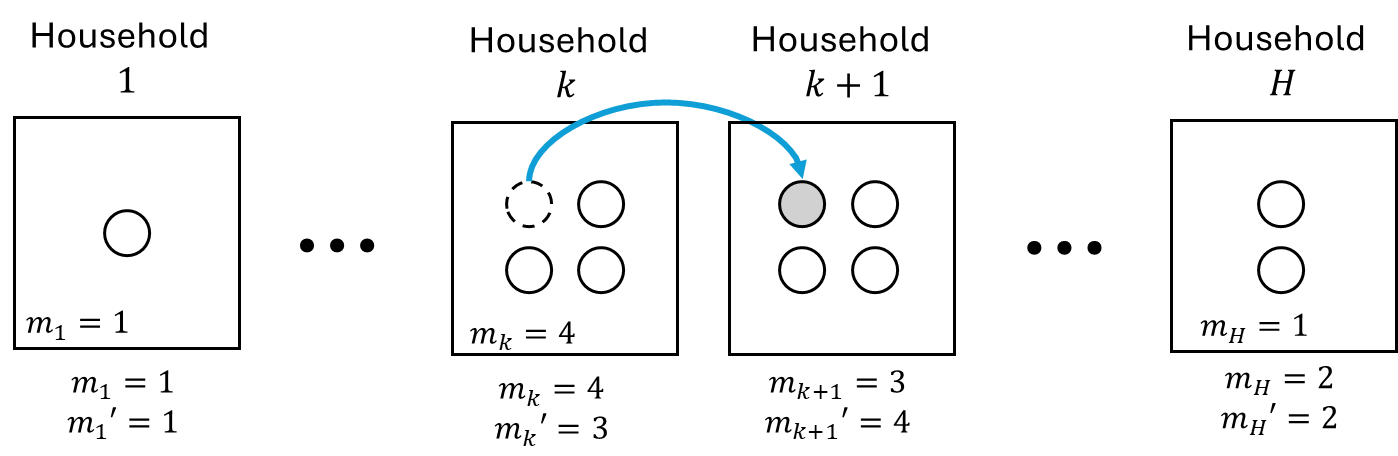
\includegraphics[width=1\linewidth]{proof_files/figure1-3}
\captionof{figure}{Initially, household $h$ has $m_k = 4$ members and household $k+1$, has $m_{k+1} = 3$ members. One individual is moved from household $k$ to household $k+1$, resulting in $m_k' = 3$ members in household $k$ and $m_{k+1}' = 4$ members in household $k+1$.}

In Case 1, the overall person-level mean household size remains
unchanged after the shift, because the two affected households have
precisely a one-person difference in their sizes. When one person moves
from the larger household to the smaller one, the decrease in the
squared size of the original larger household is exactly offset by the
increase in the squared size of the receiving household.

\begin{align}
M_p' - M_p & = \frac{1}{P} \bigg( (m_k^2 + m_{k+1}^2) - (m_k'^2 + m_{k+1}'^2) \bigg) \\
& = \frac{1}{P} \bigg( (m_k^2 + (m_k - 1)^2) - ((m_k-1)^2 + m_k^2) \bigg)\\
& = 0 \\
\end{align}

\hypertarget{case-2-a-transfer-from-a-larger-household-to-a-smaller-household}{%
\subsection{Case 2: a transfer from a larger household to a smaller
household}\label{case-2-a-transfer-from-a-larger-household-to-a-smaller-household}}

\textbf{Figure 1.4: An example single-person transfer where
\(m_{k+1} < m_k - 1\)}

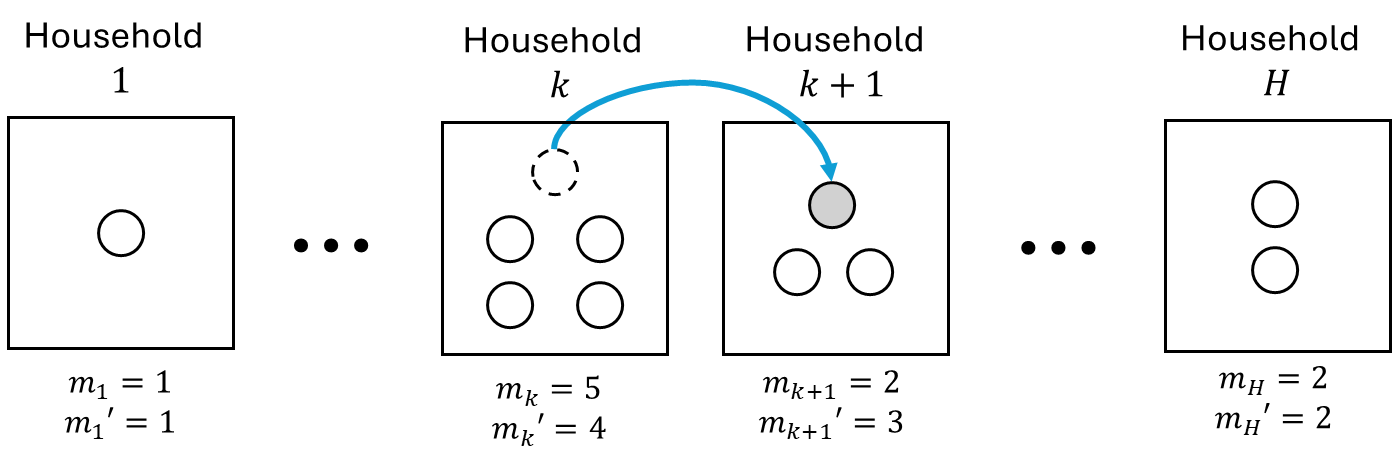
\includegraphics[width=1\linewidth]{proof_files/figure1-4}
\captionof{figure}{Initially, household $h$ has $m_k = 5$ members and household $k+1$, has $m_{k+1} = 2$ members. One individual is moved from household $k$ to household $k+1$, resulting in $m_k' = 4$ members in household $k$ and $m_{k+1}' = 3$ members in household $k+1$.}

{[}ADD IN EXPLANATION ON HOW THIS TRANSFER REDUCES AVERAGE HOUSEHOLD
SIZE{]}

\hypertarget{case-3-a-transfer-from-a-smaller-household-to-a-larger-or-equal-size-household}{%
\subsection{Case 3: a transfer from a smaller household to a larger (or
equal-size)
household}\label{case-3-a-transfer-from-a-smaller-household-to-a-larger-or-equal-size-household}}

\textbf{Figure 1.4: An example single-person transfer where
\(m_{k+1} > m_k - 1\)}

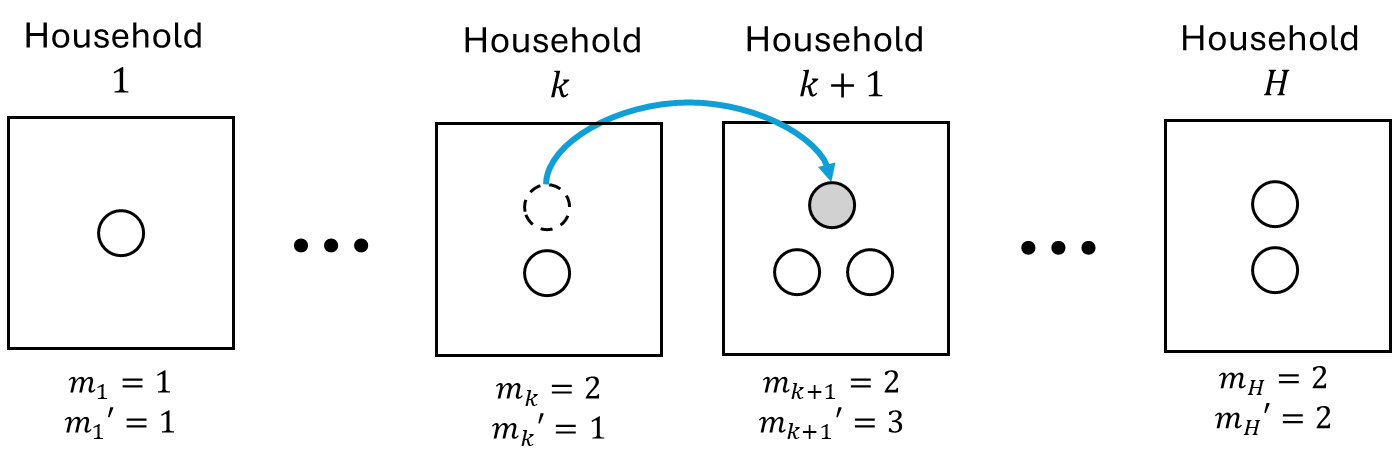
\includegraphics[width=1\linewidth]{proof_files/figure1-5}
\captionof{figure}{Initially, household $h$ has $m_k = 2$ members and household $k+1$, has $m_{k+1} = 2$ members. One individual is moved from household $k$ to household $k+1$, resulting in $m_k' = 1$ member in household $k$ and $m_{k+1}' = 3$ members in household $k+1$.}

{[}ADD IN EXPLANATION ON HOW THIS TRANSFER INCREASES AVERAGE HOUSEHOLD
SIZE{]}

\begin{center}\rule{0.5\linewidth}{0.5pt}\end{center}

{[}NEXT STEPS: Outline below, to-do more thoroughly{]}

After cases have been discussed, demonstrate that a partition of a
population into equally-sized households, each with \(m_j = M_p\), will
result in the minimal \(H\) consistent with \(M_p\). Any attempt to
further reduce number of households would require ``dissolving'' an
existing household and transferring all \(m_j\) members to other
household(s). But this would necessitate ``Case 3'' transfers, which
necessarily increase \(M_p\), as shown above. Thus, it is impossible to
formulate a configuration consistent with \(P\) and \(M_p\) that has any
fewer than \(H\) households.

{[}NOTE: Above explanation is only consistent when \(M_p\) divides
cleanly into \(P\) an integer number of times, \(i\). The proof can be
extended to cases where \(i\) is not an integer by invoking Case 1
transfers and arguing that the lowest housing configuration consistent
with \(M_p\) and \(P\) is a set of households where all
\(m_j \in \{ \lfloor M_p \rfloor, \lceil M_p \rceil \}\). And that this
exception doesn't matter anyway because the number of \(H\) that can be
constructed using
\(m_j \in \{ \lfloor M_p \rfloor, \lceil M_p \rceil \}\) such that the
population sums to \(P\) is always going to be greater than the value
\(P / M_p\).{]}

\hypertarget{lemma-2-maximum-number-of-households}{%
\section{Lemma 2: Maximum Number of
Households}\label{lemma-2-maximum-number-of-households}}

\textbf{Lemma:}\\
The maximum number of households consistent with a population size \(P\)
and person-level average household size \(M_p\) is: \begin{align}
TBD
\end{align}

\textbf{Proof:}\\
This is more of an accessory proof, since the maximum bounds on \(H\)
are so large as to not be useful in practical contexts. However, in this
section, we will demonstrate that the sparsest configuration of
households is given in a case where you produce some number of 1-person
households and then put the rest of the population into one remaining
large household. This proof will rely on Case 2 transfers, described
above.

\begin{center}\rule{0.5\linewidth}{0.5pt}\end{center}

\hypertarget{conclusion}{%
\section{conclusion}\label{conclusion}}

Reiterate the minima and maxima, take it back to the example at the
begining and show that the two configurations listed in Figure 1.2 are
actually the two special cases of minima and maxima.

\end{document}
